\chapter{Lec 06 - Decision Trees II}

\section{Inductive Bias}
Like other algorithms, ID3 can be seen as a search in a hypothesis space for a hypothesis that best fits the data. The inductive bias of ID3 consists of:
\begin{itemize}
    \item The hypothesis space: is the set of possible decision trees. The hypothesis is searched over a \textbf{subset} of DNF. This restriction is due to the fact that the root of the tree will always be the first term of the conjunction, so we can't consider the set of all the possible DNF.

    \item How the hypothesis space is explored: The search is of type \textbf{hill climbing}. ID3 starts from the empty tree and continues with more and more elaborate trees. Then, it stops when it finds a tree that is consistent with the examples. Hence, applying the information gain criterion implies that:
    \begin{itemize}
        \item Shorter trees are preferred to larger tree. This is because, at each level, it finds sets of examples with minimum entropy.
        \item Attributes with high information gain are closer to the root. 
    \end{itemize}
\end{itemize}
\section{Real-valued attributes}
Let's consider an extension of the \textit{standard} ID3 algorithm that supports also real-valued attributes.\newline\newline
Given a real-valued attribute $A$, a new \textbf{boolean} pseudo-attribute is dinamically created as:
\[A_{c} = \begin{cases}
            true & if \, \, A < c \\
            false & otherwise
          \end{cases}\]
where $c$ is a threshold.\newline\newline
Then, the content of this attribute is used to compute the information gain as the \textit{standard} ID3 does. How can we select the "\textit{correct}" value for $c$? One possibility is to select the value $c$ that provides the maximal information gain. Given the set of possible values that an attribute $A$ can take $\{v_{1},...,v_{n}\}$, the optimal value of $c$ can be proved to be always localized between two values with different labels. So, we can find the best value of $c$ looking at the information gain obtained by splitting $A$ according to $c = \frac{v_{i} + v_{i+1}}{2}$, where $v_{i}$ and $v_{i+1}$ are values that examples of the data-set with different labels have for attribute $A$.\newline\newline
Note that in this case, when we find the best attribute, differently from the case of discrete-valued ID3, that attribute it's not removed and can be used multiple times on the same path (in such case, the optimal threshold will change). We remove it only when it's not informative anymore.
\section{Attributes with missing values}
In practical applications it can happen that, for some instances, some attributes don't have a value. (missing value).\newline\newline
Given a set of examples $\hat{T}r$, when a value of an attribute $A$ is missing for an example $(x,y)$, we can:
\begin{enumerate}
    \item Assign to that missing value the most frequent value of the attribute $A$ in $\hat{T}r$.
    \item Assign the most frequent value of $A$ in $\hat{T}r$, but just considering those examples with label $y$ (of the same class).
    \item Consider the set of \textbf{distinct} values that attribute $A$ can have $V(A)$. Then, for each value $v_{i} \in V(A)$, we consider their probability of occurrence $P(v_{i}|\hat{T}r)$, estimated on $\hat{T}r$. We \textbf{substitute} the example $(x,y)$ with $|V(A)|$ \textit{fractionated examples}, one for each possible value $v_{i}$, and we weight them according to $P(v_{i}|\hat{T}r)$.
\end{enumerate}
\subsection{Handling missing values with solution 3}
Let's see an example of the behavior of the third method for handling missing values mentioned before.
\begin{center}
    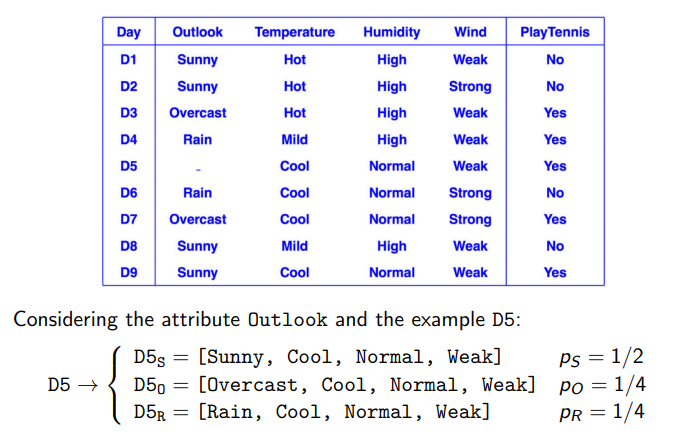
\includegraphics[]{images/Immagine 2023-01-12 152336.png}
\end{center}
As you can see, the example \textbf{D5} is substituted with three other examples (one for each distinct value of the attribute \textit{Outlook}) with their respective weights. If multiple attributes have missing values, the examples are fractionated again, and the associated weight will be the product of the weights obtained by considering the single attributes in turn.\newline\newline
In this case, we need to modify the definition of Information Gain such that the fractionated weights are considered. Basically, we compute the Information Gain using the same formula, but substituting the concept of cardinality as follows:
\[|Q| = \sum_{q \in Q}w_{q}\]
The cardinality of a set $Q$ is the sum of the weights of the examples in the set. Note that unfractionated examples will have weight 1.\newline\newline
Consider now the \textbf{classification} of a new instance that has missing values. In this case, each fractionated example is classified (using the usual classification), and, for each label, we cumulate the weights of examples classified with that label. The final classification is performed by looking at the label with the highest cumulated value.
\section{Overfitting}
A possible solution to overfitting is \textbf{Reduced-Error Pruning.}\newline\newline
Split the training set $Tr$ in $Tr^{'}$ and $Va$ (validation set), $Tr = Tr^{'} \cup Va$. Given a decision tree already learned, repeat until the performance gets worse:
\begin{enumerate}
    \item For each inner node, evaluate the accuracy in $Va$ obtained by pruning the tree on that node. We assign the label $y$ to this new leaf where $y$ is the majority label in the pruned sub-tree.
    \item If the accuracy of the new tree is higher than the \textit{original} one, return the tree.
\end{enumerate}
Another possibility is \textbf{Rule-Post Pruning:}\newline\newline
The basic idea is to turn the decision tree into a set of rules, and then do the rule pruning. A rule $R_{i}$ is generated for each path $(r, f_{i})$ from the root $r$ to the $i$-th leaf $f_{i}$. $R_{i}$ will be of the form:
\[IF(Att_{i_{1}} = v_{i_{1}}) \cap (Att_{i_{2}} = v_{i_{2}}) \cap ... (Att_{i_{k}} = v_{i_{k}}) \, THEN \, label_{f_{i}}\]
An independent pruning is carried out for each rule $R_{i}$. Basically, after removing some constraints from the preconditions of the rule, we look at the accuracy of the new rule on the validation set. If we can't improve the accuracy anymore, we return the new pruned rule. Then, the pruned $R_{i}$ are sorted in descending order of performance; eventually, add a default rule that returns the most frequent class.\newline\newline
The classification is performed following the order established for the rules:
\begin{itemize}
    \item The first rule whose preconditions are satisfied by the instance is used to classify it.
    \item If no rules have preconditions satisfied, the default rule is used to classify the instance (most frequent class).
\end{itemize}
Note that the transformation Tree $\rightarrow$ Rules \textbf{changes} the hypothesis space. We can obtain, by pruning, rules that are not expressible by a decision tree. For example, when we classify a new instance using a decision tree, we first look at the attribute attached to the root of the tree and we follow the path to a leaf according to the attributes values of the instance. But if we prune the corresponding rule at the root, the constraint of starting from the root is not present anymore.\newline\newline
Usually, Post-Rule pruning is able to improve the performance with respect to corresponding decision tree and performs better than Reduce-Error Pruning. 
